\documentclass[a4paper, 12pt]{article}%тип документа

%отступы
\usepackage[left=2cm,right=2cm,top=2cm,bottom=3cm,bindingoffset=0cm]{geometry}

%Русский язык
\usepackage[T2A]{fontenc} %кодировка
\usepackage[utf8]{inputenc} %кодировка исходного кода
\usepackage[english,russian]{babel} %локализация и переносы

%Вставка картинок
\usepackage{wrapfig}
\usepackage{graphicx}
\graphicspath{{pictures/}}
\DeclareGraphicsExtensions{.pdf,.png,.jpg}

%оглавление
\usepackage{titlesec}
\titlespacing{\chapter}{0pt}{-30pt}{12pt}
\titlespacing{\section}{\parindent}{5mm}{5mm}
\titlespacing{\subsection}{\parindent}{5mm}{5mm}
\usepackage{setspace}

%Графики
\usepackage{multirow}
\usepackage{pgfplots}
\pgfplotsset{compat=1.9}

%Математика
\usepackage{amsmath, amsfonts, amssymb, amsthm, mathtools}

%Заголовок
\author{Валеев Рауф Раушанович \\
группа 825}
\title{\textbf{Работа 1.2.2\\
Резонанс напряжений в последовательном контуре}}
\begin{document}
\maketitle
\newpage
\section*{Цель работы}
Исследование резонанса напряжений в последовательном контуре с изменяемой ёмкостью, включающее получение АЧХ и ФЧХ, а так же определение основных параметров контура.
\section*{В работе используются}
Генератор сигналов, источник напряжения, нагруженный на последовательный колебательный контур с переменной емкостью, двулучевой осциллограф, цифровые вольтметры.
\section*{Описание установки}
\begin{wrapfigure}{r}{0.5\textwidth}
	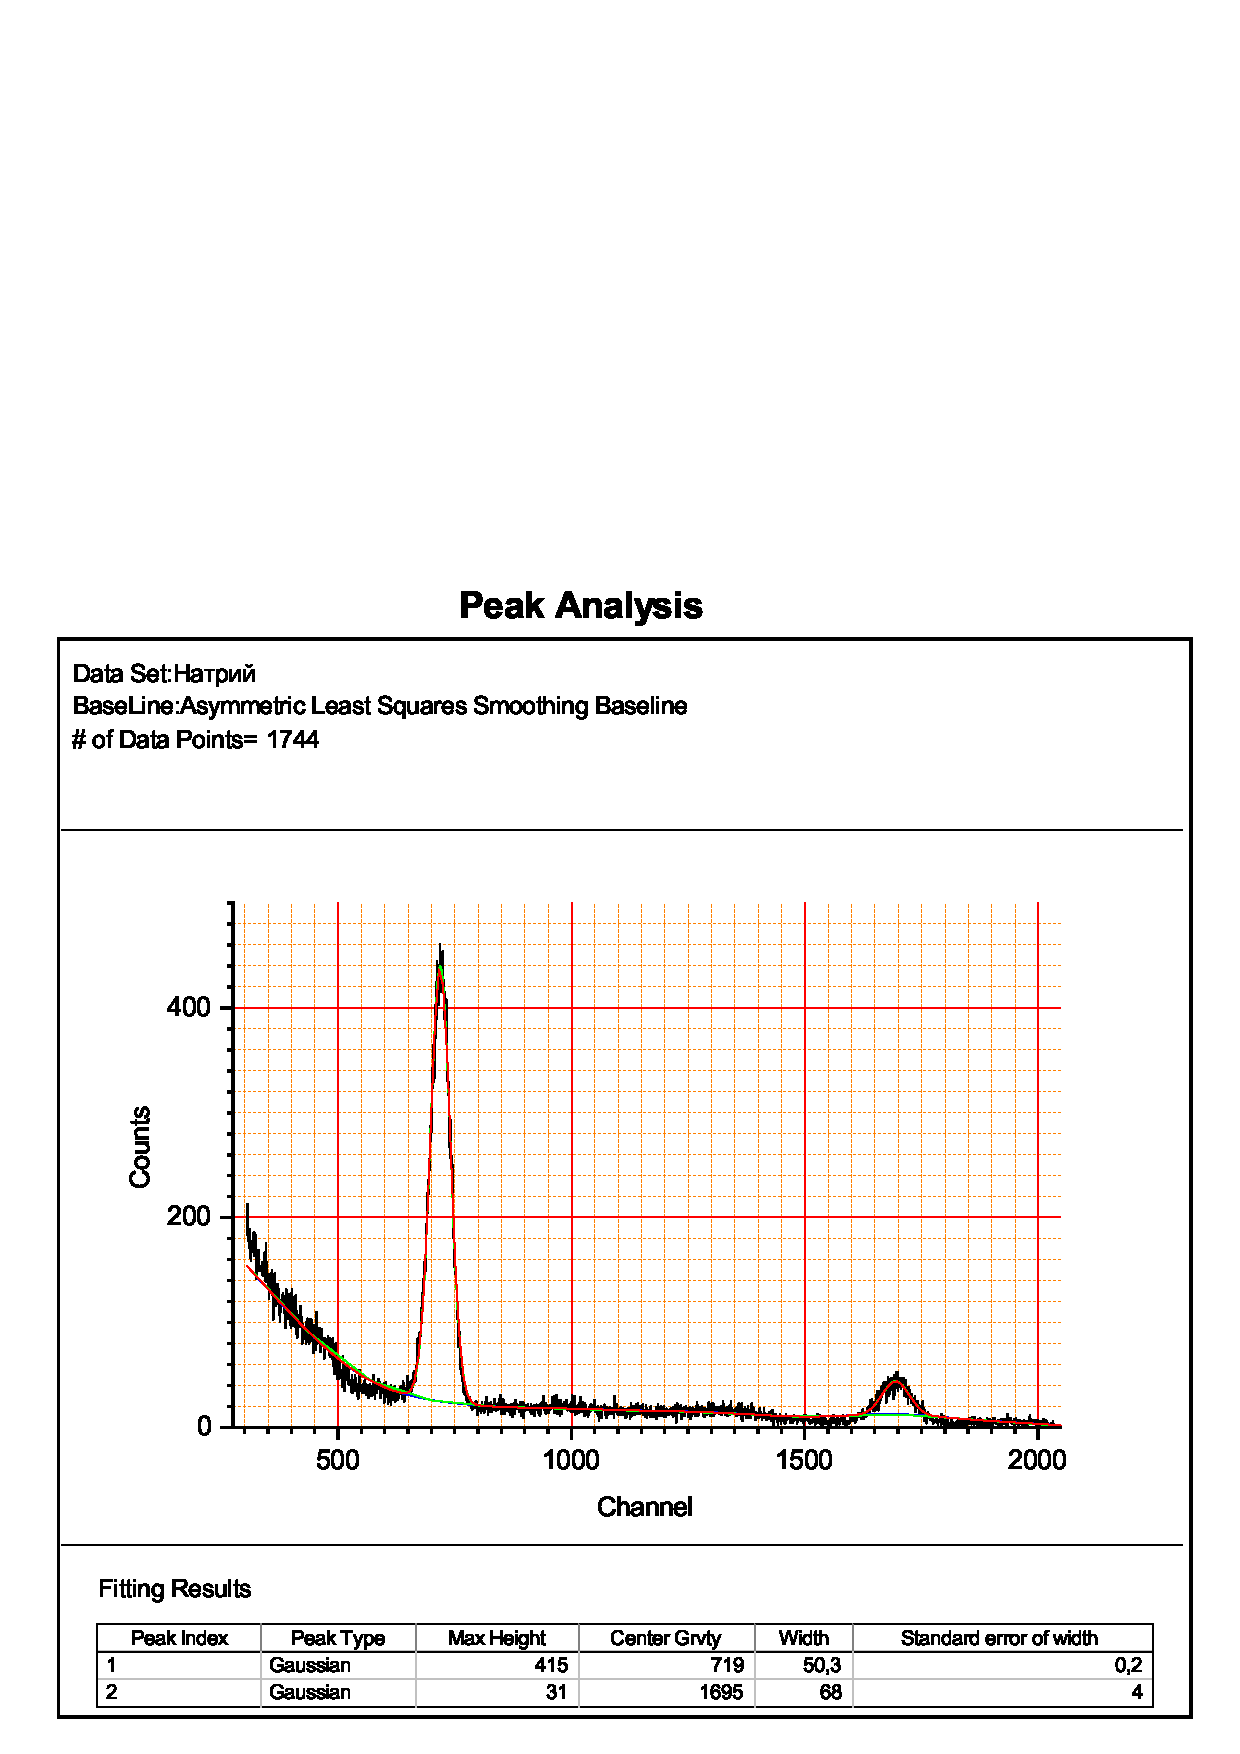
\includegraphics[width = 0.5\textwidth]{1.png}
  \textbf{\caption{Схема установки.}}
\end{wrapfigure}
Схема экспериментального стенда для изучения резонанса напряжений в последовательном колебательном контуре показана на рис. 1а. Синусоидальный сигнал от генератора GFG8255A поступает через согласующую RC-цепочку на вход источника напряжения, собранного на операционном усилителе ОУ. Питание операционного усилителя осуществляется встроенным блоком-выпрямителем от сети переменного тока 220 Вольт (цепь питания на схеме не показана). Источник напряжения, обладающий по определению нулевым внутренним сопротивлением, фактически обеспечивает с высокой точностью постоянство амплитуды сигнала $E = E_0 \cos \left(\omega t + \varphi_0\right)$ на меняющейся по величине нагрузке – последовательном колебательном контуре, изображенном на рис. 1а в виде эквивалентной схемы.
\section*{Теория}
Пусть 
\begin{equation}
R_{\sum} = R + R_S + R_L, 
\end{equation}
Здесь $R_L$ --- активное сопротивление катушки, а $R_S$ --- так называемое эквивалентное последовательное сопротивление. 
Если принять, что величины $R_L$, $C_L$ и $L$ в контуре сосредоточены в различных элементах, то можно записать следующую формулу
\begin{equation}
f_r = \dfrac{1}{2\pi \sqrt{LC_L}}
\end{equation}
Очевидно из схемы, что активные потери в конденсаторе пропорциональны $\cos \varphi$ --- сдвига фаз между током и напряжением на емкости, убывают с ростом $\varphi$ и, соответственно, с уменьшением угла $\delta = \dfrac{\pi}{2} - \varphi$. Потери в конденсаторе принято характеризовать величиной $\tg \delta$. Из схемы установки и закона Ома мы получаем, что 
\begin{equation}
R_S = \dfrac{U_{R_S}}{I} = \dfrac{U_{R_S}}{\omega C U_{C_S}} = \dfrac{1}{\omega C}\tg\delta
\end{equation}
Далее будем пользоваться методом комплексных амплитуд 
\begin{equation}
Z_L = R_L + i\omega L, Z_C = R_S - \dfrac{i}{\omega C}, Z = R_{\sum} + i \left(\omega L - \dfrac{1}{\omega C}\right)
\end{equation}
Комплексные амплитуды тока в контуре и напряжений на индуктивности и емкости при нулевой начальной фазе удобно представить в виде 
\begin{equation}
\begin{gathered}
\vec{I} = \dfrac{E}{R_{\sum}} \dfrac{1}{1 + iQ	\left(\dfrac{\omega}{\omega_0} - \dfrac{\omega_0}{\omega} \right)}\\
\vec{U_L} = iEQ \dfrac{\omega}{\omega_0} \dfrac{1 - iR_L/\rho}{1 + iQ\left(\dfrac{\omega}{\omega_0} - \dfrac{\omega_0}{\omega} \right)}\\
\vec{U_C} = -iEQ\dfrac{\omega_0}{\omega} \dfrac{1 + i\tg \delta}{1 + iQ\left(\dfrac{\omega}{\omega_0} - \dfrac{\omega_0}{\omega} \right)}
\end{gathered}
\end{equation}
Здесь использованы стандартные обозначения $\omega_0 = \dfrac{1}{\sqrt{LC}}$ --- собственная частота, и $\rho = \sqrt{\dfrac{L}{C}}$ --- реактивное сопротивление, $Q$ --- добротность, связанная с его параметрами соотношением 
\begin{equation}
Q = \dfrac{\rho}{R_{\sum}} = \dfrac{\omega_0 L}{R_{\sum}} = \dfrac{1}{\omega_0CR_{\sum}} \gg 1
\end{equation}
При резонансе, когда $\omega = \omega_0$, выражение для модулей комплексных амплитуд принимают вид
\begin{equation}
\begin{gathered}
I(\omega_0) = \dfrac{E}{R_{\sum}}, \varphi_I(\omega_0) = 0\\
U_L(\omega_0) = QE, \varphi_L(\omega_0) = \dfrac{\pi}{2} - \dfrac{R_L}{\rho}\\
U_C(\omega_0) = QE, \varphi_C(\omega_0) - \dfrac{\pi}{2} + \delta
\end{gathered}
\end{equation}
\begin{equation}
Q = \left(\dfrac{\Delta f}{f_0}\right)^{-1},
\end{equation}
где $\Delta f$ - разность частот на $U_C(f) = \dfrac{U_C(f)}{\sqrt{2}}$, аналогично можно определить и по разности фаз между точками, где фаза $\varphi_C$ меняется от $-\dfrac{\pi}{4}$ до $-\dfrac{3\pi}{4}$
\newpage
\section*{Ход работы}
Измеряем резонансные частоты и напряжения. Резонанс отслеживаем по фигурам Лиссажу, так как на них главные оси элипса будут направлены вдоль осей X, Y. \\
\begin{center}
\begin{tabular}{|c|c|c|c|c|c|c|c|}
\hline
$n$                                                                             & 1    & 2    & 3    & 4    & 5    & 6    & 7    \\ \hline
$C_n$, пФ                                                                       & 25,0 & 33,2 & 47,5 & 57,2 & 67,4 & 82,1 & 99,6 \\ \hline
$\sigma_{C_n}$, пФ                                                              & 0,1  & 0,1  & 0,1  & 0,1  & 0,1  & 0,1  & 0,1  \\ \hline
$f_{\text{резонанс}}$, кГц                                                      & 32,0 & 28,0 & 23,3 & 21,2 & 19,6 & 17,7 & 16,2 \\ \hline
$\sigma_{f_{\text{резонанс}}}$,   кГц & 0,1  & 0,1  & 0,1  & 0,1  & 0,1  & 0,1  & 0,1  \\ \hline
$U$, В                                                                          & 2,57 & 2,14 & 1,98 & 1,831 & 1,700 & 1,571 & 1,441 \\ \hline
$\sigma_U$, В                                                                   & 0,02 & 0,02 & 0,02 & 0,018 & 0,017 & 0,016 & 0,015 \\ \hline
\end{tabular}\\
\textbf{Таблица 1.} Значения резонансных частот и напряжений.
\end{center}
Далее следует из формул $(1)-(8)$ в более явном виде записать формулы необходимых нам величин:
\begin{equation}
\begin{gathered}
L = \dfrac{1}{4\pi^2f_{0n}^2C}\\
Q = \dfrac{f_{0n}}{\Delta f}\\
\rho = \sqrt{\dfrac{L}{C}}\\
R_{\sum} = \rho \tg \delta\\
R_{S_{\max}} = 10^{-3}\rho\\
R_S = \dfrac{1}{\omega C} \tg \delta\\
R_L = R_{\sum} - R - R_S\\
I = \dfrac{E}{R_{\sum}}
\end{gathered}
\end{equation}
\newpage
Далее считаем АЧХ для двух конденсаторов $C_1$ и $C_2$\\
В данном опыте приборные погрешности равны $\sigma_f = 0,1$ Гц и $\sigma_A = 0,01$ В.
\begin{center}
\begin{tabular}{ccc|c|c|c|}
\hline
\multicolumn{3}{|c|}{$C_1 = (25,0\pm 0,1)$ нФ}                                                                                                         & \multicolumn{3}{c|}{$C_4 = (57,2 \pm 0,1)$ нФ}        \\ \hline
\multicolumn{1}{|c|}{$n$} & \multicolumn{1}{c|}{$f$, кГц}  & \multicolumn{1}{c|}{$A$, В}   & $n$ & f, кГц & $A$ , В  \\ \hline
\multicolumn{1}{|c|}{1}   & \multicolumn{1}{c|}{29,8}  & \multicolumn{1}{c|}{0,40}                  & 1   & 17     & 0,13          \\ \hline
\multicolumn{1}{|c|}{2}   & \multicolumn{1}{c|}{27,3}                & \multicolumn{1}{c|}{0,20}                    & 2   & 17,6    & 0,18  \\ \hline
\multicolumn{1}{|c|}{3}   & \multicolumn{1}{c|}{28}                   & \multicolumn{1}{c|}{0,22}                    & 3   & 18,4                & 0,22         \\ \hline
\multicolumn{1}{|c|}{4}   & \multicolumn{1}{c|}{28,5}            & \multicolumn{1}{c|}{0,25}                   & 4   & 18,7             & 0,24          \\ \hline
\multicolumn{1}{|c|}{5}   & \multicolumn{1}{c|}{29}             & \multicolumn{1}{c|}{0,28}                   & 5   & 19                 & 0,26          \\ \hline
\multicolumn{1}{|c|}{6}   & \multicolumn{1}{c|}{29,5}          & \multicolumn{1}{c|}{0,32}                   & 6   & 19,3             & 0,30    \\ \hline
\multicolumn{1}{|c|}{7}   & \multicolumn{1}{c|}{30,5}          & \multicolumn{1}{c|}{0,48}                   & 7   & 19,5            & 0,32      \\ \hline
\multicolumn{1}{|c|}{8}   & \multicolumn{1}{c|}{30,9}              & \multicolumn{1}{c|}{0,60}                  & 8   & 19,7               & 0,34 \\ \hline
\multicolumn{1}{|c|}{9}   & \multicolumn{1}{c|}{31,3}        & \multicolumn{1}{c|}{0,90}                 & 9   & 20                 & 0,4  \\ \hline
\multicolumn{1}{|c|}{10}  & \multicolumn{1}{c|}{31,5}  & \multicolumn{1}{c|}{1,00}                 & 10  & 20,2             & 0,48          \\ \hline
\multicolumn{1}{|c|}{11}  & \multicolumn{1}{c|}{31,7}  & \multicolumn{1}{c|}{1,10}                & 11  & 20,3             & 0,52         \\ \hline
\multicolumn{1}{|c|}{12}  & \multicolumn{1}{c|}{31,9}   & \multicolumn{1}{c|}{1,30}        & 12  & 20,5          & 0,6      \\ \hline
\multicolumn{1}{|c|}{13}  & \multicolumn{1}{c|}{32}         & \multicolumn{1}{c|}{1,40}           & 13  & 20,7           & 0,78      \\ \hline
\multicolumn{1}{|c|}{14}  & \multicolumn{1}{c|}{32,2}    & \multicolumn{1}{c|}{1,35}                  & 14  & 20,8            & 0,83         \\ \hline
\multicolumn{1}{|c|}{15}  & \multicolumn{1}{c|}{32,4}           & \multicolumn{1}{c|}{1,25}     & 15  & 21,1           & 1,00         \\ \hline
\multicolumn{1}{|c|}{16}  & \multicolumn{1}{c|}{32,8}   & \multicolumn{1}{c|}{0,90}               & 16  & 21,2              & 1,00           \\ \hline
\multicolumn{1}{|c|}{17}  & \multicolumn{1}{c|}{33,1}         & \multicolumn{1}{c|}{0,75}                  & 17  & 21,4               & 1,00         \\ \hline
\multicolumn{1}{|c|}{18}  & \multicolumn{1}{c|}{33,6}                 & \multicolumn{1}{c|}{0,60}                  & 18  & 21,6            & 0,80      \\ \hline
\multicolumn{1}{|c|}{19}  & \multicolumn{1}{c|}{34,1}      & \multicolumn{1}{c|}{0,40}                  & 19  & 21,8               & 0,72         \\ \hline
\multicolumn{1}{|c|}{20}  & \multicolumn{1}{c|}{34,6}          & \multicolumn{1}{c|}{0,35}      & 20  & 21,9           & 0,64         \\ \hline
\multicolumn{1}{|c|}{21}  & \multicolumn{1}{c|}{35,1}           & \multicolumn{1}{c|}{0,24}              & 21  & 22,1           & 0,54         \\ \hline
\multicolumn{1}{|c|}{22}  & \multicolumn{1}{c|}{35,4}          & \multicolumn{1}{c|}{0,24}             & 22  & 22,6              & 0,4          \\ \hline
\multicolumn{1}{|c|}{23}  & \multicolumn{1}{c|}{36,6}              & \multicolumn{1}{c|}{0,18}                   & 23  & 22,9        & 0,32          \\ \hline
\multicolumn{1}{|c|}{24}  & \multicolumn{1}{c|}{37,3}           & \multicolumn{1}{c|}{0,16}       & 24  & 23,2     & 0,28 \\ \hline
\multicolumn{1}{|c|}{25}  & \multicolumn{1}{c|}{32,5}      & \multicolumn{1}{c|}{1,30}    & 25  & 23,6   & 0,24 \\ \hline
\multicolumn{1}{|c|}{26}  & \multicolumn{1}{c|}{32,9}  & \multicolumn{1}{c|}{0,85}  & 26  & 23,8  & 0,22 \\ \hline
\multicolumn{1}{|c|}{27}  & \multicolumn{1}{c|}{33}        & \multicolumn{1}{c|}{0,80}  & 27  & 24,3  & 0,18  \\ \hline
 \multicolumn{1}{l}{}                 & \multicolumn{1}{l}{}        & \multicolumn{1}{l|}{} & 28  & 24,6           & 0,16         \\ \cline{4-6} 
\multicolumn{1}{l}{}           & \multicolumn{1}{l}{}        & \multicolumn{1}{l|}{} & 29  & 24,9      & 0,15  \\ \cline{4-6} 
\end{tabular}\\
\textbf{Таблица 2.} АЧХ для двух конденсаторов $C_1$ и $C_2$.
\end{center}
\newpage
Строим графики по полученным данным, один из которых строим в безразмерных осях. Из последнего мы получим $Q$.\\
\begin{center}
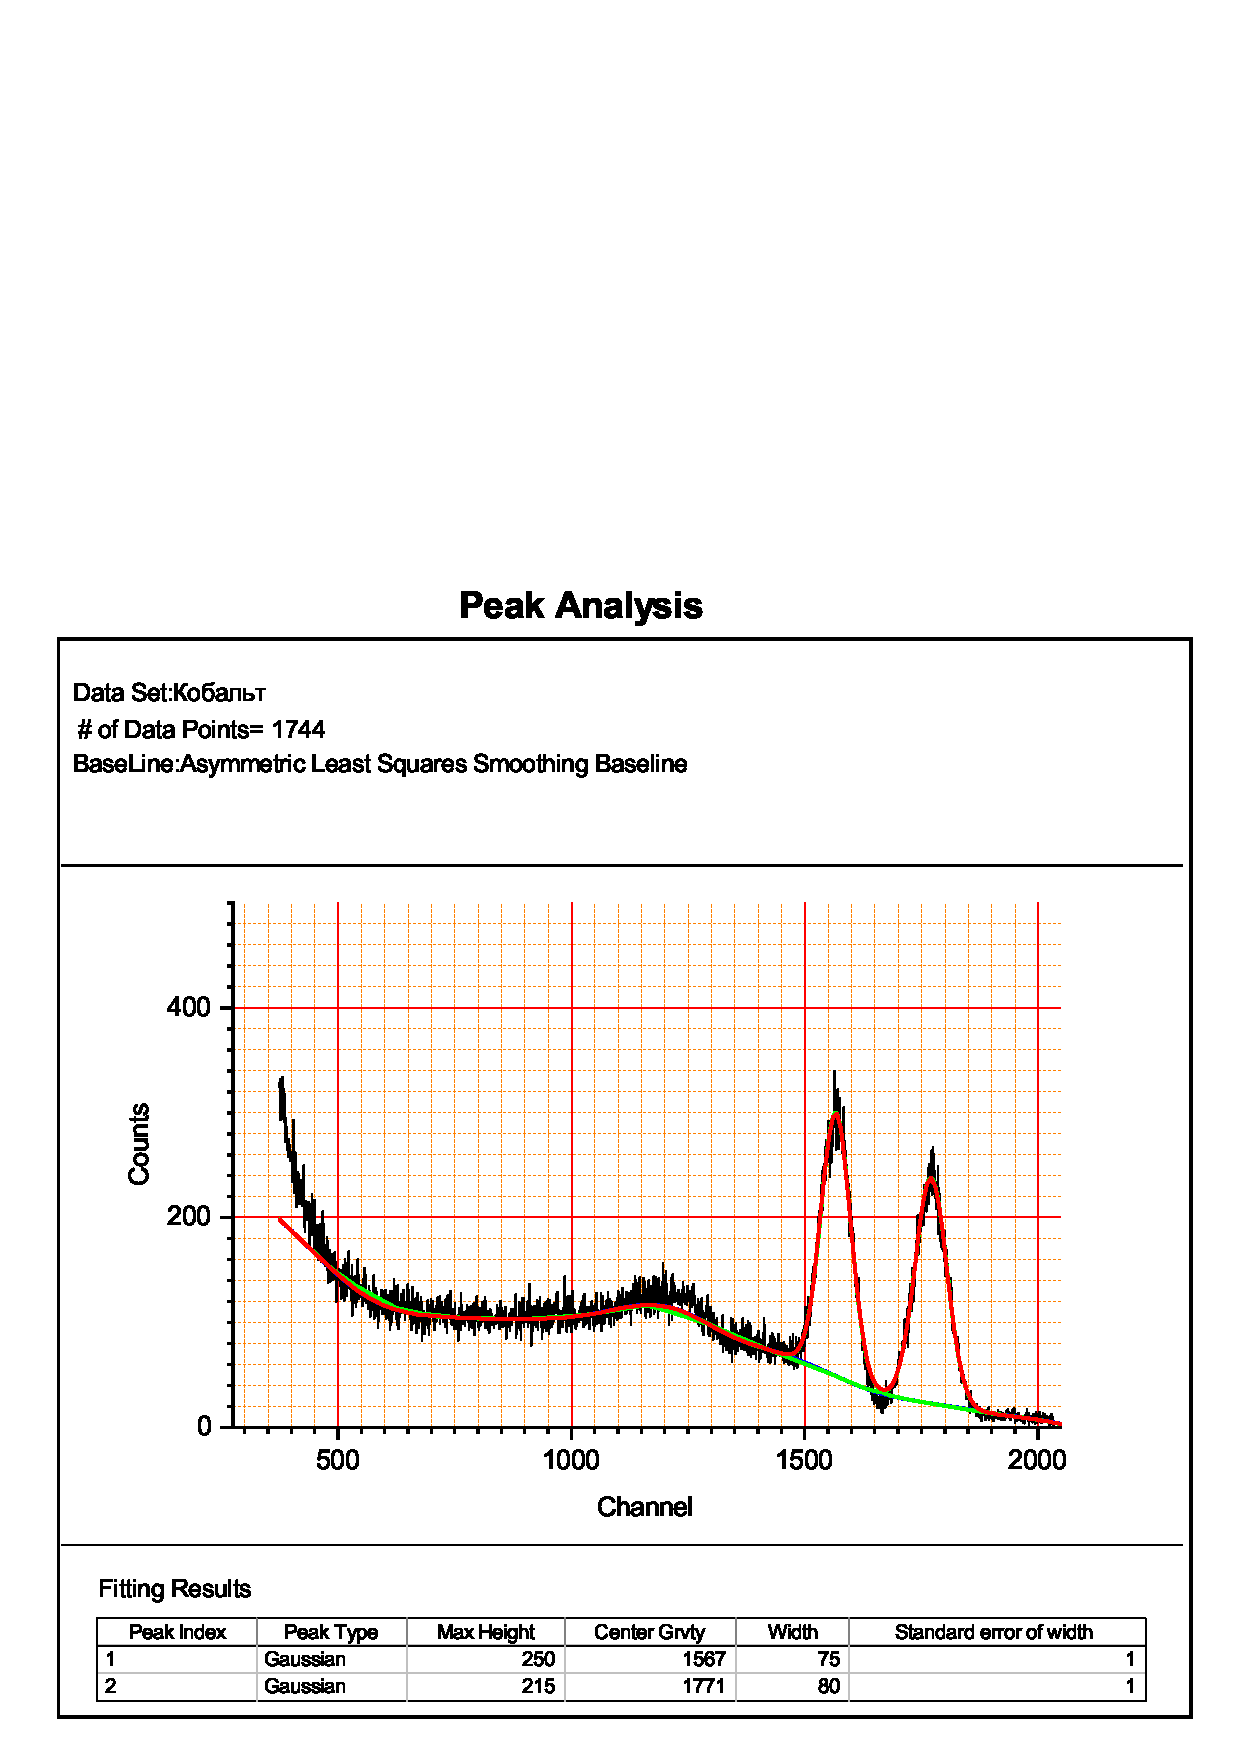
\includegraphics[width = 0.8\textwidth]{2.jpg}\\
\textbf{График 1.} АЧХ в координатах с размерностями.
\end{center}
\begin{center}
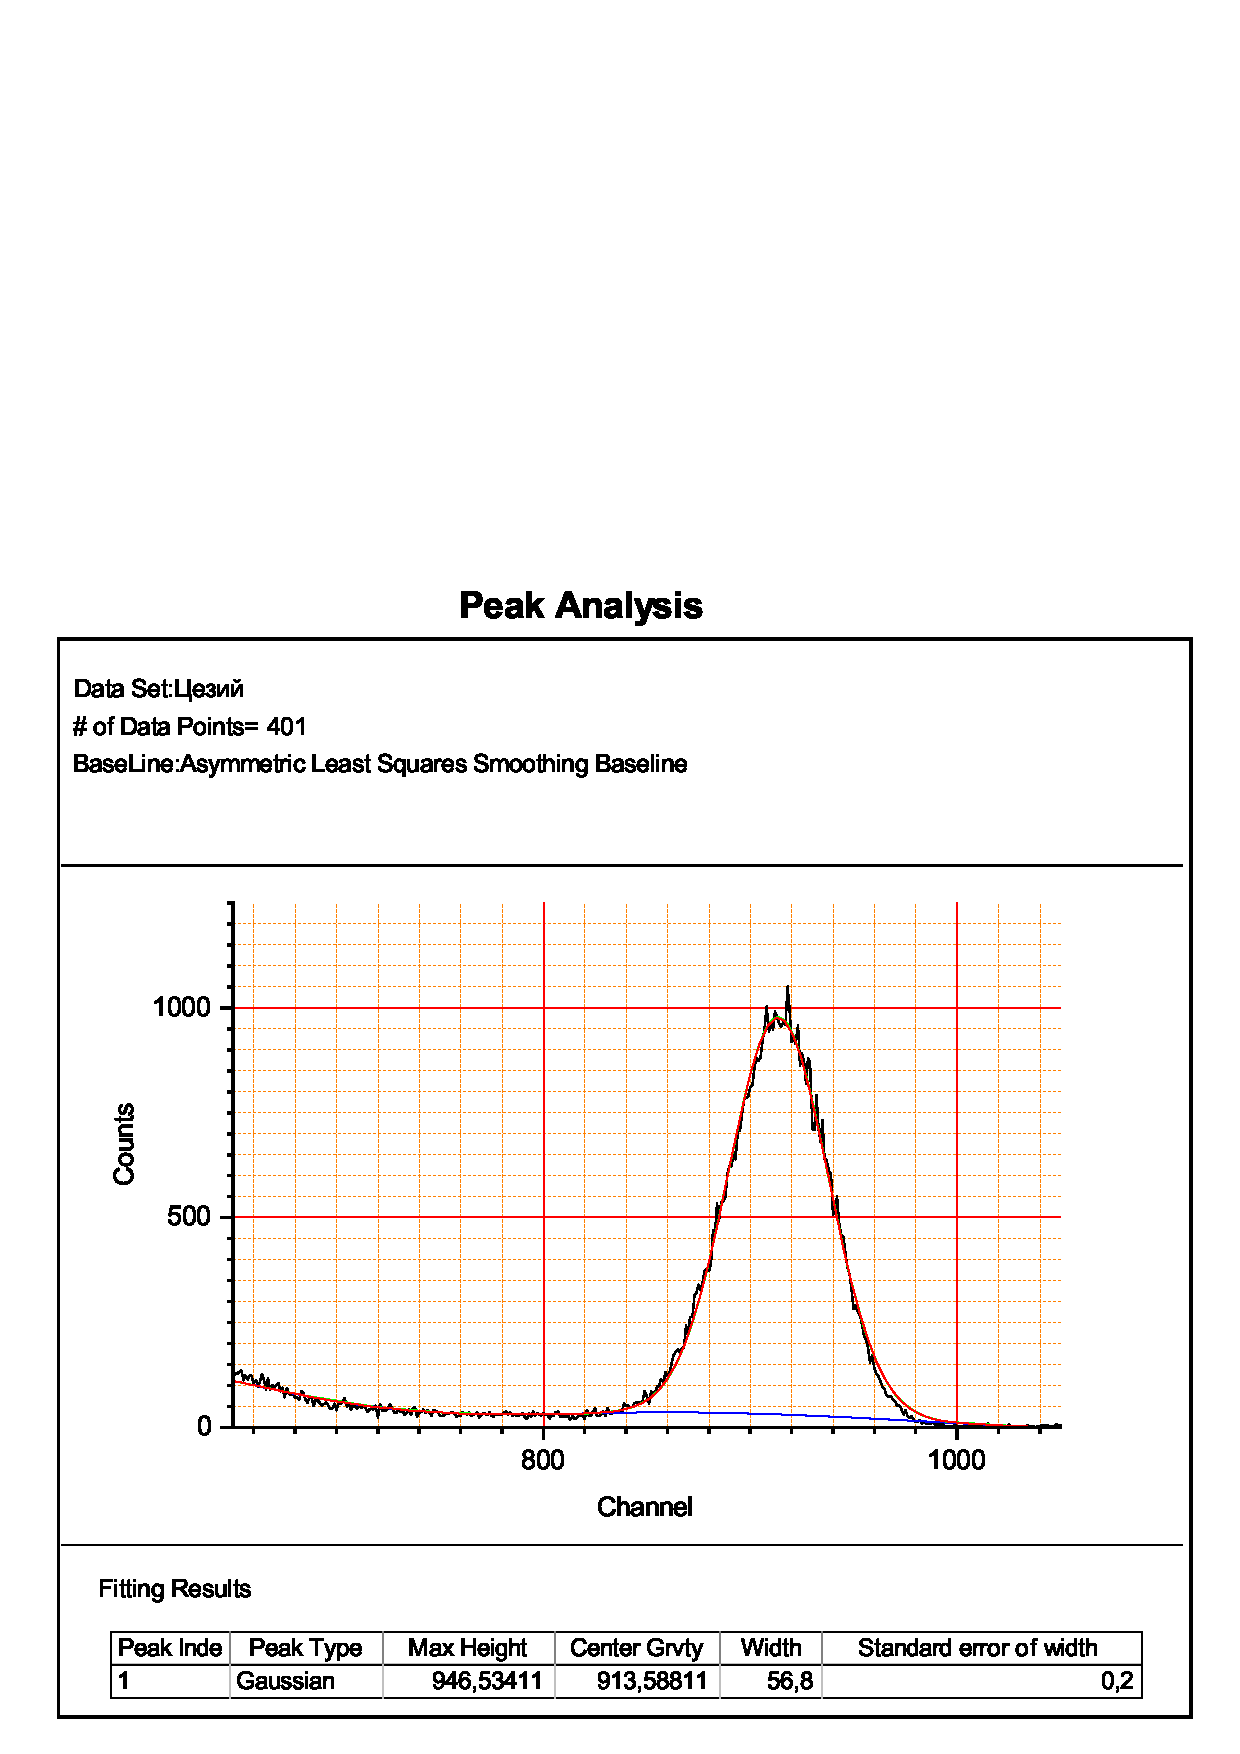
\includegraphics[width = 0.8\textwidth]{3.jpg}\\
\textbf{График 2.} АЧХ в безразмерных координатах.
\end{center}
Из этих графиков мы находим $Q \approx 25 \pm 5$.\\
Теперь заполним таблицу, состоящую из величин, из формулы $(9)$\\
\begin{center}
\begin{tabular}{|c|c|c|c|c|c|c|c|c|c|c|c|}
\hline
$n$ & $C_n$, нФ & \begin{tabular}[c]{@{}c@{}}$f_{0n}$, \\ кГц\end{tabular} & $U_C$, В & $E$, В & \begin{tabular}[c]{@{}c@{}}$L$, \\ мкГн\end{tabular} & $Q$ & \begin{tabular}[c]{@{}c@{}}$\rho$, \\ Ом\end{tabular} & \begin{tabular}[c]{@{}c@{}}$R_{\sum}$, \\ Ом\end{tabular} & \begin{tabular}[c]{@{}c@{}}$R_{S_{\max}}$,\\ Ом\end{tabular} & $R_L$, Ом & $I$, мА \\ \hline
1 & 25,0 & 32,0 & 2,57 & 0,1 & 991 & 25 & 199 & 12,6 & 0,201 & 8,9 & 8,01 \\ \hline
2 & 33,2 & 28,0 & 2,14 & 0,1 & 975 & 25 & 171 & 10,8 & 0,173 & 7,2 & 9,30 \\ \hline
3 & 47,5 & 23,3 & 1,98 & 0,1 & 984 & 25 & 144 & 9,1 & 0,141 & 5,5 & 11,03 \\ \hline
4 & 57,2 & 21,2 & 1,83 & 0,1 & 987 & 25 & 131 & 8,3 & 0,137 & 4,7 & 12,11 \\ \hline
5 & 67,4 & 19,6 & 1,70 & 0,1 & 980 & 25 & 121 & 7,6 & 0,124 & 4 & 13,22 \\ \hline
6 & 82,1 & 17,7 & 1,57 & 0,1 & 986 & 25 & 110 & 6,9 & 0,112 & 3,4 & 14,53 \\ \hline
7 & 99,6 & 16,2 & 1,44 & 0,1 & 971 & 25 & 99 & 6,2 & 0,100 & 2,7 & 16,12 \\ \hline
\multicolumn{5}{|c|}{Среднее значение} & 982 & \multicolumn{4}{c|}{--} & 5 & -- \\ \hline
\multicolumn{5}{|c|}{\begin{tabular}[c]{@{}c@{}}Среднеквадратичная погрешность\\ среднего значения\end{tabular}} & 3 & \multicolumn{4}{c|}{--} & 1 & -- \\ \hline
\multicolumn{5}{|c|}{\begin{tabular}[c]{@{}c@{}}Коэффициент Стьюденса\\ $t_{n \alpha}$ для\\ $n = 7$, $\alpha = 0,95$\end{tabular}} & 2,34 & \multicolumn{4}{c|}{--} & 2,34 & -- \\ \hline
\multicolumn{5}{|c|}{Случайная погрешность} & 6 & \multicolumn{4}{c|}{--} & 2 & -- \\ \hline
\end{tabular}\\
\textbf{Таблица 3.} Данные об основных величинах установки.\\
\end{center}
Теперь построим график ФЧХ.\\
\begin{center}
\includegraphics[width = 0.9\textwidth]{4.jpg}\\
\textbf{График 3.} ФЧХ для двух конденсаторов $C_1$, $C_4$
\end{center}
Поскольку мы меряем $\varphi$ по осциллографу считая относительно исходного пи, так же померяного по осцилографу, которое по значению порядка 3 клеток, а на осциллографе у клеток погрешность $\sigma_{osc} = 0,1$, то мы можем считать погрешность $\sigma_{\varphi \cdot \pi} \approx 0,03$, а $\sigma_f = 0,1$. 
\begin{center}
\begin{tabular}{ccc||c|c|c|}
\hline
\multicolumn{3}{|c||}{$C_4 = (25,0 \pm 0,1)$ нФ} & \multicolumn{3}{c|}{$C_4 = (57,2 \pm 0,1)$ нФ} \\ \hline
\multicolumn{1}{|c|}{$n$} & \multicolumn{1}{c|}{$f$, кГц} & $-\varphi\cdot \pi$ & $n$ & $f$, кГц & $-\varphi\cdot \pi$ \\ \hline
\multicolumn{1}{|c|}{1} & \multicolumn{1}{c|}{29,6} & 0,03 & 1 & 18,8 & 0,06 \\ \hline
\multicolumn{1}{|c|}{2} & \multicolumn{1}{c|}{29,8} & 0,04 & 2 & 19,0 & 0,08 \\ \hline
\multicolumn{1}{|c|}{3} & \multicolumn{1}{c|}{30,0} & 0,05 & 3 & 19,5 & 0,08 \\ \hline
\multicolumn{1}{|c|}{4} & \multicolumn{1}{c|}{30,4} & 0,05 & 4 & 19,6 & 0,11 \\ \hline
\multicolumn{1}{|c|}{5} & \multicolumn{1}{c|}{30,8} & 0,10 & 5 & 19,8 & 0,15 \\ \hline
\multicolumn{1}{|c|}{6} & \multicolumn{1}{c|}{31,2} & 0,14 & 6 & 20,1 & 0,17 \\ \hline
\multicolumn{1}{|c|}{7} & \multicolumn{1}{c|}{31,5} & 0,21 & 7 & 20,3 & 0,20 \\ \hline
\multicolumn{1}{|c|}{8} & \multicolumn{1}{c|}{31,6} & 0,29 & 8 & 20,5 & 0,22 \\ \hline
\multicolumn{1}{|c|}{9} & \multicolumn{1}{c|}{31,9} & 0,40 & 9 & 20,7 & 0,27 \\ \hline
\multicolumn{1}{|c|}{10} & \multicolumn{1}{c|}{32,0} & 0,49 & 10 & 20,8 & 0,36 \\ \hline
\multicolumn{1}{|c|}{11} & \multicolumn{1}{c|}{32,3} & 0,60 & 11 & 21,0 & 0,41 \\ \hline
\multicolumn{1}{|c|}{12} & \multicolumn{1}{c|}{32,5} & 0,71 & 12 & 21,1 & 0,45 \\ \hline
\multicolumn{1}{|c|}{13} & \multicolumn{1}{c|}{32,8} & 0,80 & 13 & 21,2 & 0,48 \\ \hline
\multicolumn{1}{|c|}{14} & \multicolumn{1}{c|}{33,0} & 0,86 & 14 & 21,3 & 0,57 \\ \hline
\multicolumn{1}{|c|}{15} & \multicolumn{1}{c|}{33,2} & 0,87 & 15 & 21,5 & 0,71 \\ \hline
\multicolumn{1}{|c|}{16} & \multicolumn{1}{c|}{33,5} & 0,88 & 16 & 21,7 & 0,81 \\ \hline
\multicolumn{1}{|c|}{17} & \multicolumn{1}{c|}{33,8} & 0,94 & 17 & 22,0 & 0,86 \\ \hline
\multicolumn{1}{|c|}{18} & \multicolumn{1}{c|}{34,0} & 0,98 & 18 & 22,3 & 0,93 \\ \hline
\multicolumn{1}{|c|}{19} & \multicolumn{1}{c|}{34,4} & 1,00 & 19 & 22,4 & 1,00 \\ \hline
\multicolumn{1}{|c|}{20} & \multicolumn{1}{c|}{32,6} & 0,74 & 20 & 22,6 & 1,11 \\ \hline
\multicolumn{1}{|c|}{21} & \multicolumn{1}{c|}{32,4} & 0,66 & 21 & 22,8 & 1,00 \\ \hline
 &  &  & 22 & 23,1 & 0,98 \\ \cline{4-6} 
\end{tabular}\\
\textbf{Таблица 4.} Данные ФЧХ.
\end{center}
По всем вышеперечисленным характеристикам мы можем определить добротность, запишем в таблицу.
\begin{center}
\begin{tabular}{|c|c|c|}
\hline
Измерение & $n$ к-ра & $Q$ \\ \hline
\multirow{2}{*}{АЧХ} & 1 & 25 \\ \cline{2-3} 
 & 2 & 18 \\ \hline
\multirow{2}{*}{ФЧХ} & 1 & 25 \\ \cline{2-3} 
 & 2 & 33 \\ \hline
\multicolumn{2}{|c|}{Ср. знач.} & 25 \\ \hline
\multicolumn{2}{|c|}{Ср-кв. откл.} & 3 \\ \hline
\end{tabular}\\
\textbf{Таблица 5.} Добротность
\end{center}
Построим по данным таблицы 3 зависимость $R_L(f_{0n})$, на этом же графике построим $<R_L>$\\
\begin{center}
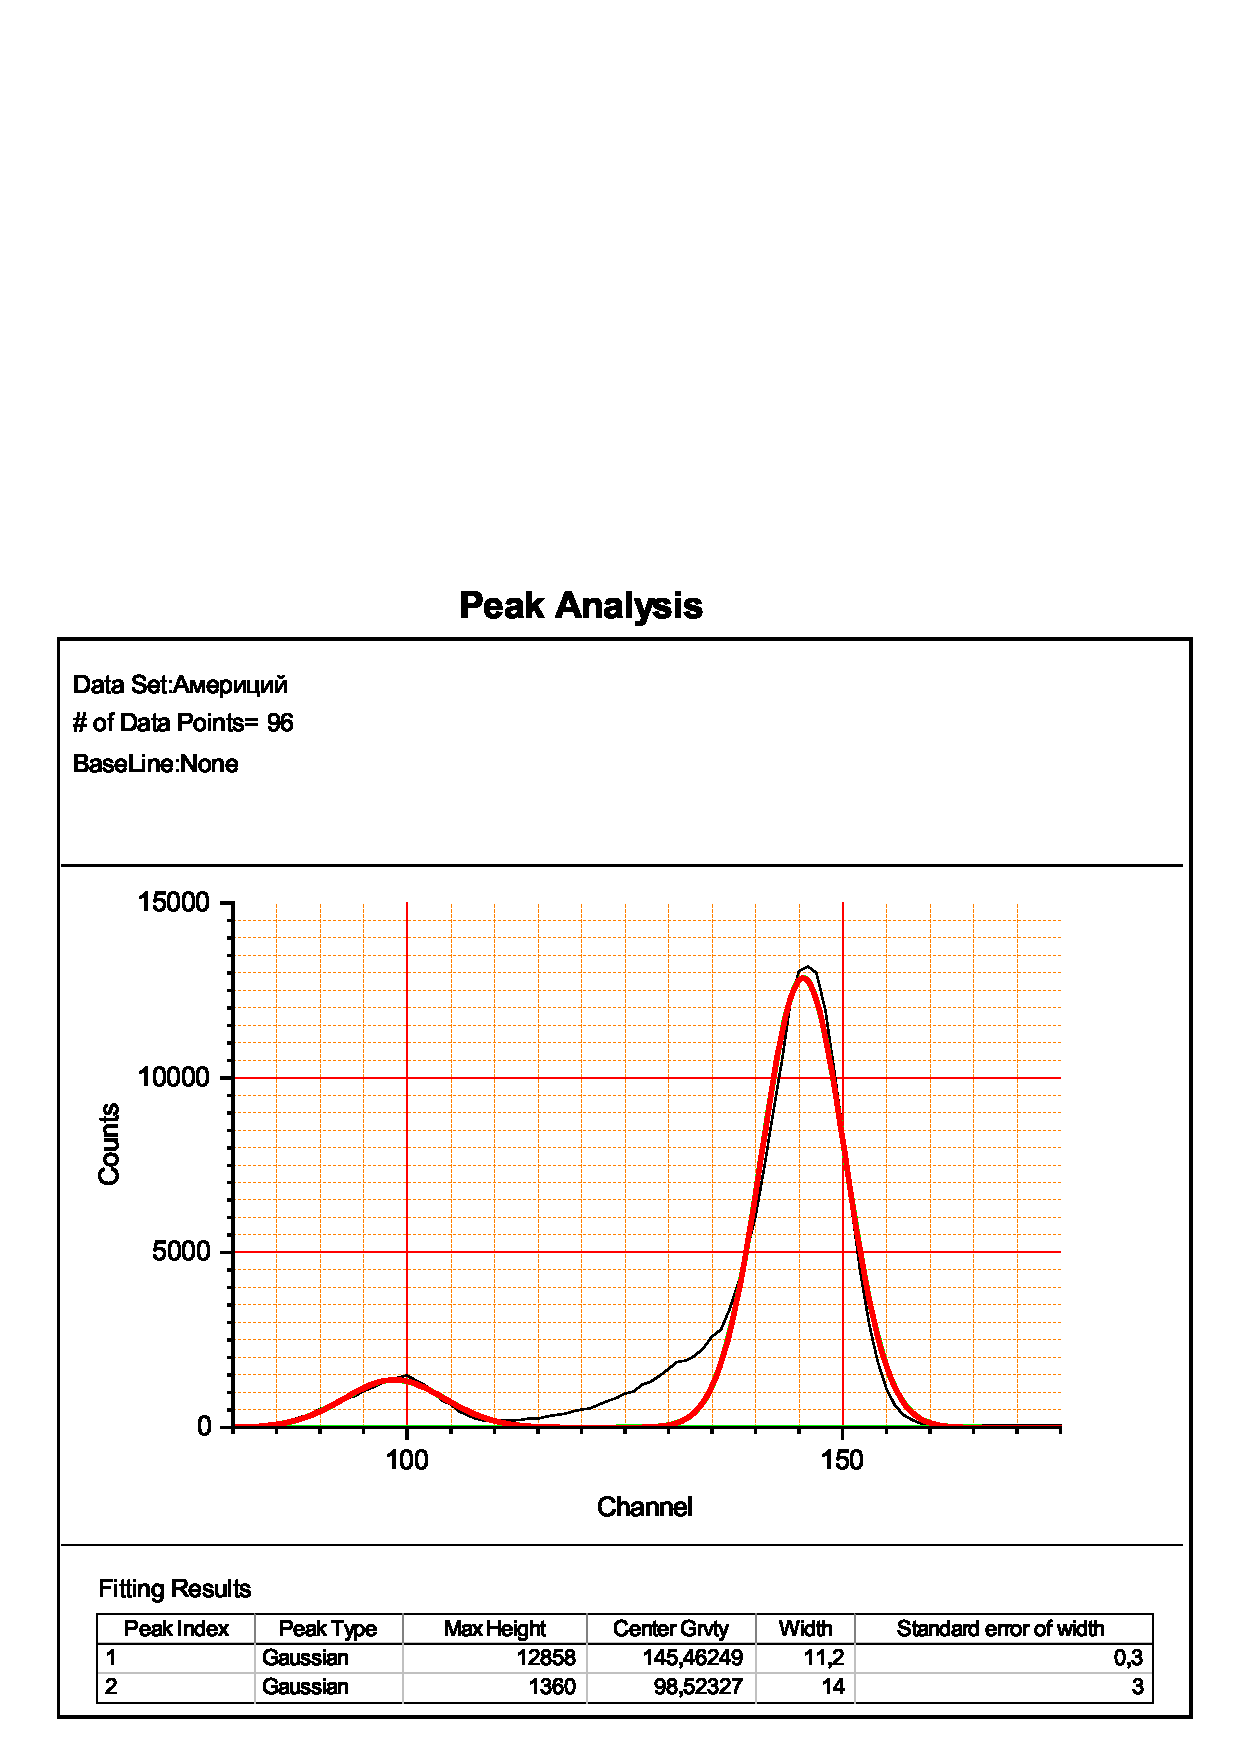
\includegraphics[width = \textwidth]{5.jpg}\\
  \textbf{График 4.} Зависимость $R_L(f_{0n})$\\
\end{center}
Из графика видно, что $R_L$ линейно растет с частой резонансной. Эту зависимость можно связать с линейной зависимостью
\[Z_L = \omega \cdot L\]
\section*{Литература}
\begin{enumerate}
\item \textbf{Лабораторный практикум по общей физике:} Учебное пособие. В трех томах. Т. 2. Электричество и магнетизм /Гладун А.Д., Александров Д.А., Берулёва Н.С. и др.; Под ред. А.Д. Гладуна - М.: МФТИ, 2007. - 280 с.
\item \textbf{Дополнительное описание лабораторной работы 1.2.2}: Резонанс напряжений; Под ред. МФТИ, 2017. - 10 с.
\end{enumerate}
\end{document}
